\section{Решение}
Кривая строится с некоторой точностью, берем угол $\phi$ с некоторым шагом, заполняя массив пар значениями функции и углом, далее преобразованием
\[
\systeme*{x = \rho * cos(2 * \pi * i / n), y = \rho * cos(2 * \pi * i / n)}
\]
n - точность разбиения, i $\in$ (0, n). Далее следует преобразование смещения и масштабирования для дальнейшей отрисовки на плоскости.

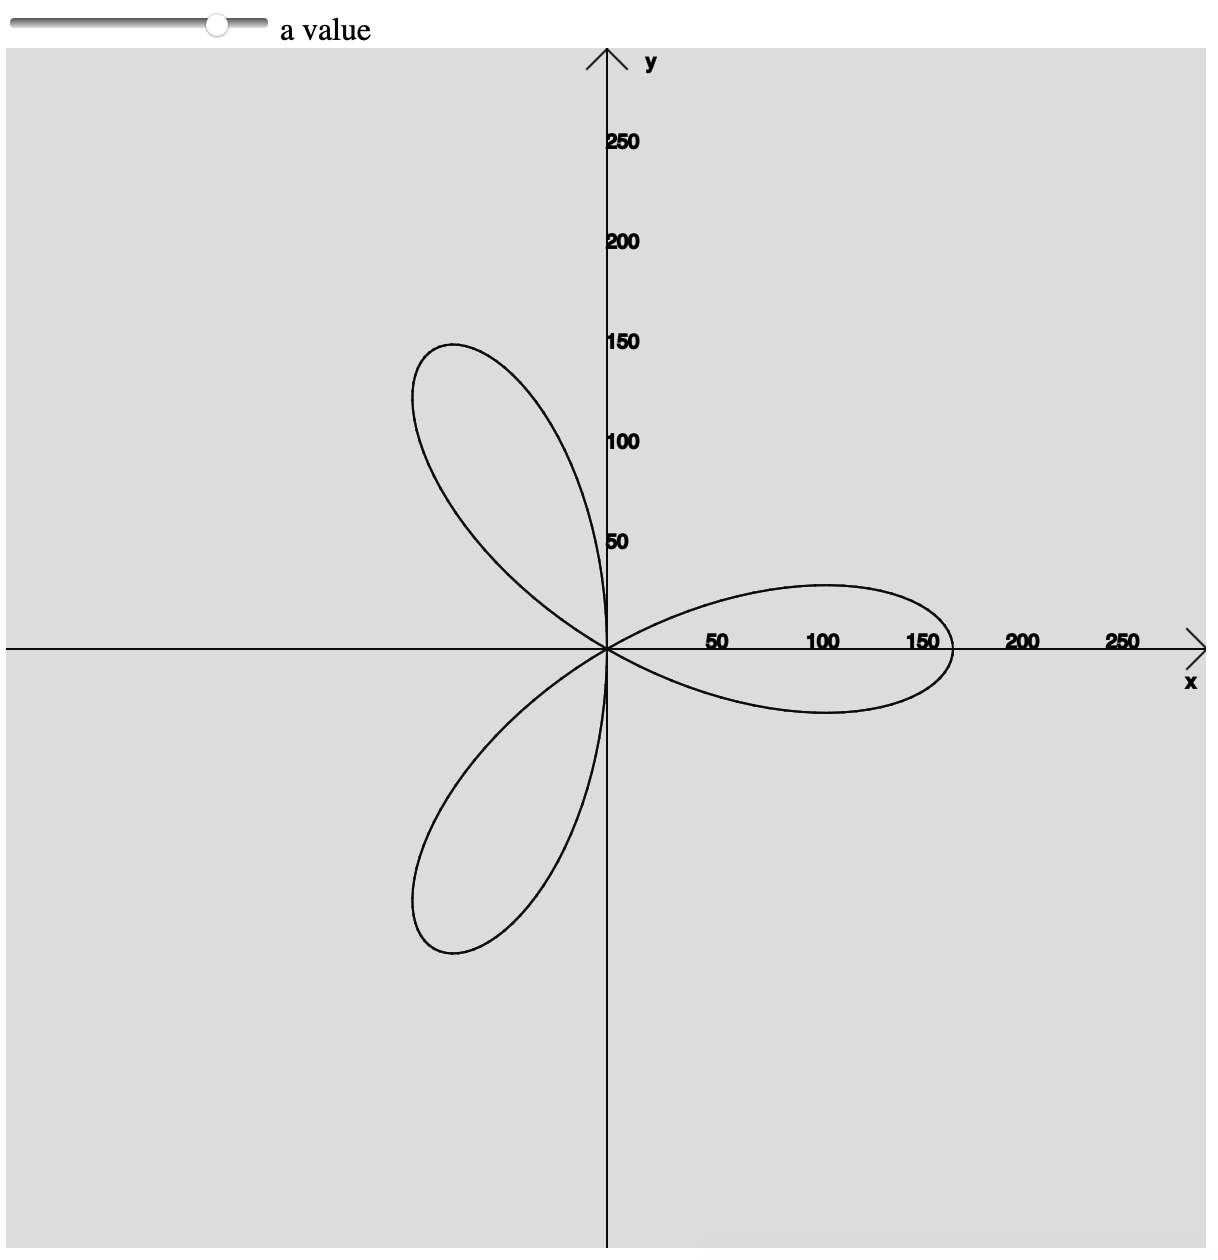
\includegraphics[scale=0.5]{pictures/1.png}

Ползунком a value регулируется параментр a в кривой, динамически меняя ее отображение.

% \section{Исходный код}

% \begin{lstlisting}[language=C++]
% \end{lstlisting}

% \lstset{language=[gnu] make}
% \lstset{
%   language=[gnu] make,
%   keywordstyle=\color{teal}\textbf,
%   stringstyle=\color{blue},
%   identifierstyle=\itshape
% }

% \begin{lstlisting}
% CC = g++
% CCFLAGS = -std=c++14 -Wall -pedantic -O3
% ###____###
% solution : main.cpp *.hpp ; $(CC) $(CCFLAGS) main.cpp -o solution
% clean	 : ;
% \end{lstlisting}

% \section{Консоль}

% \begin{alltt}
% \end{alltt}

% \pagebreak